\chapter{Regulatory Framework}
\label{ch:regulatory_framework}

The regulatory framework governing drones is a complex and dynamic area, influenced by various laws and regulations that differ from country to country. Generally, drone operations are regulated by aviation authorities responsible for ensuring safe and responsible usage.

\section{Relevant Institutions}

\subsection{\glsentryfull{easa}}
The \gls{easa} \autocite{eu-1139-2018} plays a crucial role in harmonizing aviation safety standards across all \gls{eu} member states. Its primary objective is to maintain a consistent and high level of safety in civil aviation operations throughout the \gls{eu}. \gls{easa} achieves this through the establishment and enforcement of common regulations applicable to all member states. Notably, for the standardization of \gls{uas}, \gls{easa} has implemented Regulations (EU) 2019/947 \autocite{eu-947-2019} and (EU) 2019/945 \autocite{eu-945-2019}.

\subsection{\glsentryfull{aesa}}
In Spain, the \gls{aesa} \autocite{sp-184-2008} serves as the national regulatory authority, overseeing compliance with civil aviation standards within the aerospace sector. \gls{aesa} plays a critical role in promoting the development and application of aviation legislation, ensuring that the Spanish civil aviation system upholds the highest safety, quality, and sustainability standards. In instances of non-compliance with aviation regulations, \gls{aesa} possesses the authority to enforce sanctions.

\section{Applicable Legislation}

\subsection{Implementing Regulation (EU) 2019/947}
The Implementing Regulation (EU) 2019/947 \autocite{eu-947-2019} establishes the operational rules and requirements for UAS within the \gls{eu}. It provides a legal framework for the utilization of \gls{uas} across various operational categories, outlining requirements for operational authorizations and risk assessments where applicable. The regulation sets standards for remote pilot competency, operational procedures, and safety management to conduct \gls{uas} flights safely and effectively.

Additionally, it integrates with the Delegated Regulation (EU) 2019/945 \autocite{eu-945-2019} by defining operational requirements related to the \gls{uas} classes established within it. The regulation details specific operational limitations and conditions for each \gls{uas} class, including the management of \gls{uas} in classes C0 through C4. It also includes provisions for the safe integration of newly introduced \gls{uas} classes under Delegated Regulation (EU) 2020/1058 \autocite{eu-1058-2020}, specifically classes C5 and C6.

Moreover, this regulation addresses the procedures for \gls{uas} operators from third countries (non-\gls{easa} member states) wishing to operate within the \gls{ses} airspace, ensuring alignment with \gls{eu} standards and safety regulations.

\subsection{Delegated Regulation (EU) 2019/945}
The Delegated Regulation (EU) 2019/945 \autocite{eu-945-2019} defines the rules and standards for \gls{uas} within the \gls{eu}. It specifies the types of \gls{uas} that require certification regarding design, production, and maintenance. This regulation also provides guidelines for the commercialization of \gls{uas} intended for use in the Open category, as well as for remote identification accessories (e.g., Drone Remote ID). Furthermore, it outlines the requirements for the design and manufacture of \gls{uas} intended for operations defined in the Implementing Regulation (EU) 2019/947.

\subsection{Regulation (EU) 2024/1689: \glsentryfull{ai_act}}
The \gls{ai_act} of the \gls{eu} \autocite{AIActIntoForce}, which came into force on the 1st of August 2024, aims to ensure that \gls{ai} systems are safe, transparent, and ethical, while fostering innovation and protecting fundamental rights as stated in the Delegated Regulation (EU) 2024/1689 \autocite{eu-1689-2024}. The \gls{ai_act} categorizes \gls{ai} systems by risk, imposing strict requirements on high-risk applications, particularly in aviation, which may affect public safety and fundamental rights. These requirements encompass robust risk management, transparency, human oversight, and data governance, ensuring that \gls{ai} systems are reliable and secure.

The \gls{ai_act} introduces significant compliance obligations that could escalate development costs and timelines. High-risk systems must adhere to stringent standards to access the \gls{eu} market, potentially challenging innovation but ultimately aiming to build trust and facilitate broader adoption of \gls{ai} technologies within the \gls{eu}.

\section{Operational Categories}
The Regulation (EU) 2019/947 \autocite{eu-947-2019} classifies \gls{uas} into three distinct categories:

\begin{itemize}
  \item \textbf{Open Category:} The least restrictive category, designed for low-risk operations, includes activities such as recreational flying and commercial operations posing minimal risk to people and property. Operators must adhere to specific limitations (e.g., flying below 120 meters, maintaining \gls{vlos}). \gls{uas} must weigh under 25 kg, and pilots must ensure that the drone does not fly over people or in restricted areas. No prior authorization is required, though registration and remote pilot training are compulsory for all operations, except for drones weighing less than 250 g that lack a camera or sensor.

  \item \textbf{Specific Category:} This category covers medium-risk operations necessitating a more detailed assessment. It includes operations that may involve flying over people or in restricted areas, provided mitigation procedures are in place. Operators must conduct a risk assessment and obtain an operational authorization known as \gls{sts} from \gls{aesa}. Requirements for \gls{uas} and pilot qualifications may vary based on the specific risk assessment and operational procedures defined within it.

  \item \textbf{Certified Category:} Designed for high-risk operations, this category involves stringent requirements comparable to those for manned aviation. \gls{uas} must meet specific certification standards and operators must comply with strict safety regulations. This category often includes advanced training requirements and operational procedures similar to those for commercial air transport.
\end{itemize}

\subsection{Open Category}
This work will focus on civil \gls{uas} that fall under \gls{easa}'s Open Category, although some findings may be applicable to other categories with appropriate regulatory adjustments. Within the Open Category, three subcategories differentiate based on associated risk, aircraft weight, and operational limits:

\begin{enumerate}
  \item \textbf{A1}: \gls{uas} with a \gls{mtow} of less than 250 g that can fly over people but not over assemblies of people.

  \item \textbf{A2}: \gls{uas} with an \gls{mtow} of less than 4 kg that can fly close to people but must maintain a horizontal distance of 30 meters (5 meters in low-speed configuration).

  \item \textbf{A3}: \gls{uas} with an \gls{mtow} of less than 25 kg that must maintain a horizontal distance of 150 meters from residential, commercial, industrial, or recreational areas.
\end{enumerate}

Check \cref{fig:eu_regulations_open_category_chart} for a visual representationof the Open Category subcategories.

\begin{figure}
  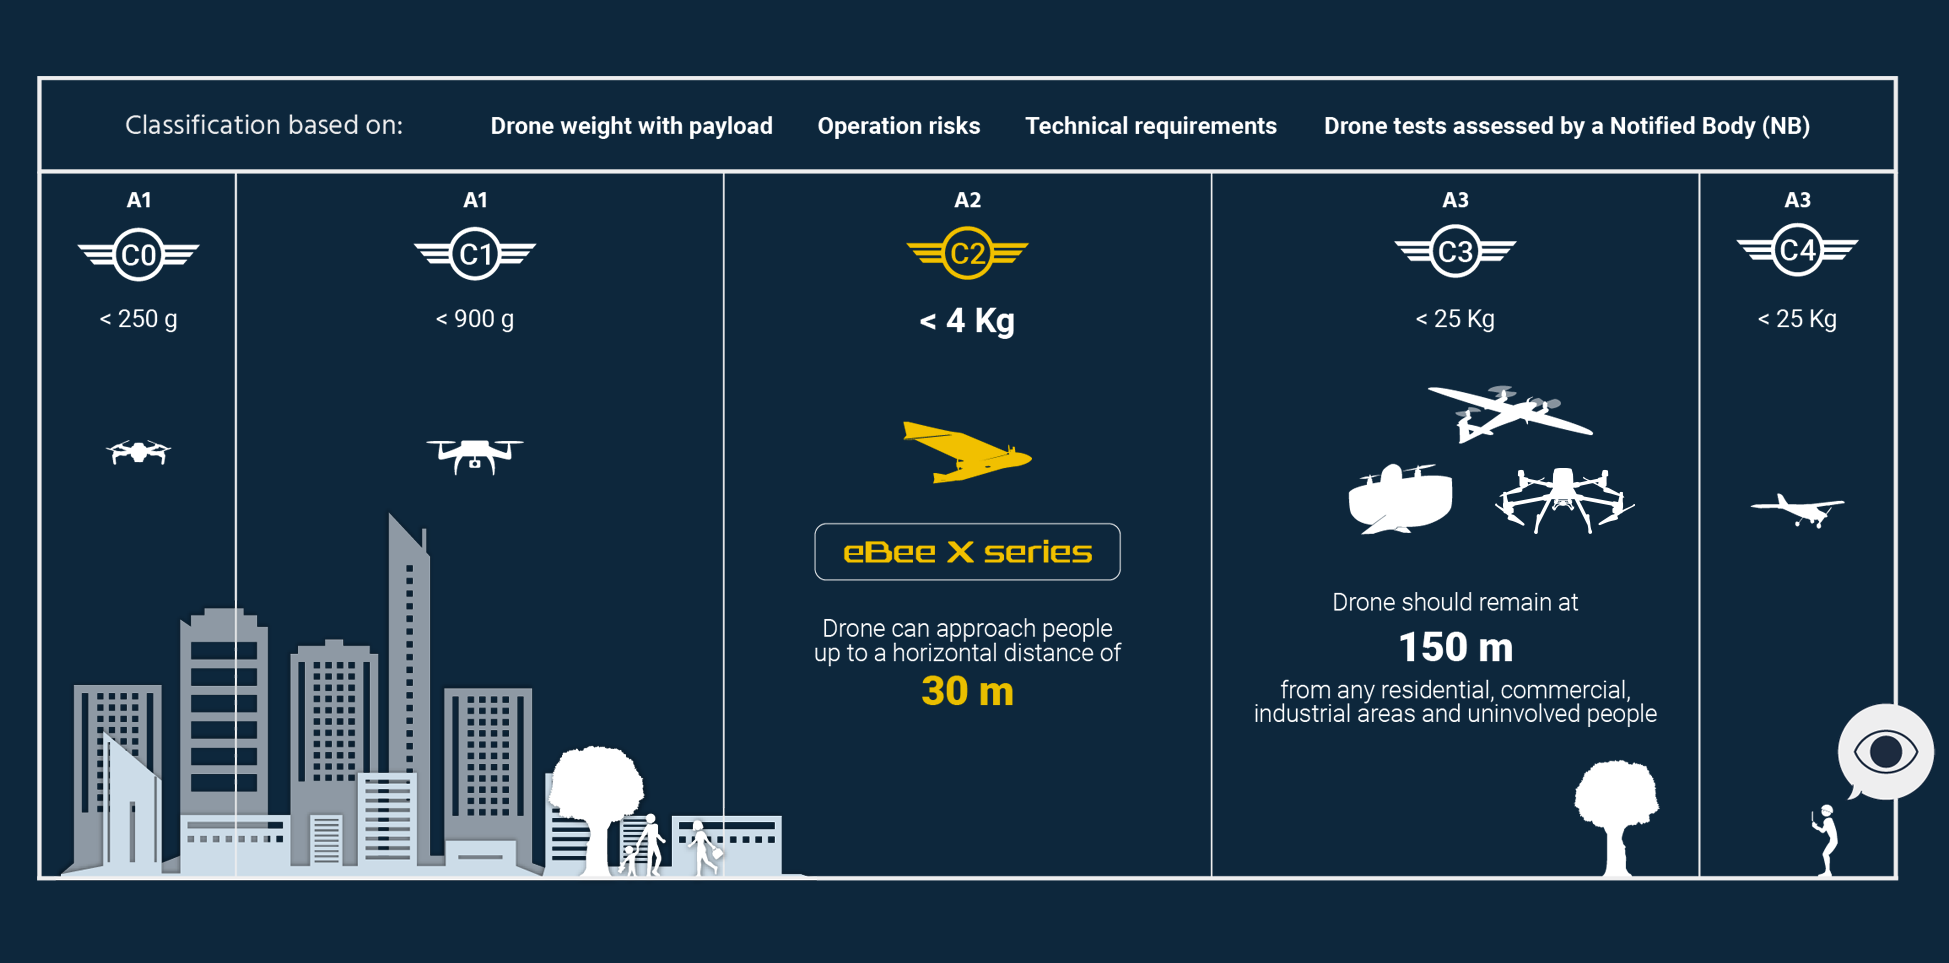
\includegraphics{eu_regulations_open_category_chart.png}
  \caption{\glsentryshort{eu} Regulations Open Category chart describing the subcategories A1, A2, and A3 with their respective operational limitations \autocite{ageagleEuropeanUnion}}
  \label{fig:eu_regulations_open_category_chart}
\end{figure}

Moreover, additional rules applicable to all three subcategories include:

\begin{itemize}
  \item The maximum height must not exceed 120 meters above ground level, as the lower limit for general aviation is 150 meters. This leaves only a 30-meter separation between manned aviation and UAS.

  \item Operators must always maintain \gls{vlos} unless the aircraft is in ``follow me'' mode or the pilot is using \gls{fpv} goggles.

  \item Operators must register if the \gls{uas} weighs more than 250 g or if the aircraft is equipped with a camera or sensor.

  \item The aircraft must possess a remote identification ID, which is standard in all C1-C6 categories, with the exception of C4 and privately built aircraft.
\end{itemize}
